% put environments that should be ignored by texcount here, e.g., here lstlisting for code

%TC:envir lstlisting [] ignore

%for reference to this section
\section{Introduction}
\label{section:Introduction}

The aim of this paper is to get a correlation between pedestrian traffic and route satisfaction. Given an open GPS Trajectories Dataset from the OpenStreetMap Project the research was conducted on the historical walking data in the city of Salzburg in Austria. Due to the historical growth of the city, footpaths, and pedestrian areas along with roads for private and public transport are limited to change and urban development (SOURCE). 

Historical traffic pattern mining and analysis for traffic forecasting and improving traffic flow is nothing new to vehicle traffic management. Multiple studies focus on collecting data, analyzing patterns, and forecasting traffic flow for vehicle traffic. 

Is it possible to increase satisfaction by recommending alternative, less populated routes to tourist attractions using pedestrian path model techniques?

This template is used for seminar papers, bachelor and master theses at MultiMediaTechnology of the Salzburg University of Applied Sciences. 

The structure of the template fits many theses works. Seminar papers often require their own structure as it is a literature review on a specific topic and does not present your own work.

Outline the research field and lead towards your research question. How is the investigated issue resolved in related work? What are limitations of these solutions? What is your contribution to find a solution?

The purpose of the research is to study the development of the concept of actorness in the literature and apply it to the European Union by studying and comparing the actorness of the last in the spheres of energy and environment

The structure of the thesis goes as follows: the literature review elaborates on the main definition of the research, namely actorness, its characteristics, as well as the actorness of the EU in the energy and environmental sphere. Chapter I reveals the development of the EU energy policy as a shared competence, adds clearness to the concept of actorness in the present context, and discusses the basic European and international legislation and the changes brought by it. Chapter II examines the history of the environmental policy of the EU and reveals the Union’s actorness in this regard. The conclusion of the thesis compares the EU actorness in the energy and environmental sphere and tries to predict the further developments and the challenges of the issue in question.

\section{Background}
Lorem ipsum dolor sit amet, consectetur adipiscing elit. Morbi luctus lacinia sagittis. Maecenas vestibulum ex quam, eget placerat mi pharetra ut. Cras molestie lectus eget efficitur sagittis. Ut porttitor lobortis odio, eget commodo velit consectetur vitae. Quisque ornare auctor neque eleifend bibendum. Praesent molestie efficitur pulvinar. Nullam lobortis lacus sit amet mi tempor, sed suscipit dolor euismod. Pellentesque eget orci eget risus pharetra sodales sed vel nunc. Praesent consequat urna eu libero vestibulum porttitor.


\section{Related Work}
Introduce why this specific related work is important for your own work. Which areas do you cover and why? What do you take as inspiration and what do you do differently/improve upon? 

\autocite[]{Sevtsuk2021}
  

\section{Method}

To be able to measure a possible increase in satisfaction of the route proposal a qualitative trail run will be conducted. In this trail run a standard route will be compared to the newly proposed route and measured by using two surveys. Survey number one is using a quantitative approach to find out the subjects general travel behavior while survey number two is there to compare and measure the satisfaction with a quantitative approach after conducting the trail run.

Finding out about the subjects travel behavior should give a better understanding of the results from the route proposal satisfaction survey. Furthermore it is going to give a relation to the subjects travel behavior and the increase or decrease in satisfaction.

Qualitative Surveys.

Proposing said alternative route will be done by using the influence of historical pedestrian traffic to calculate a route with less interactions for the traveler to get to the same goal. This is going to be done by analysing historical GPS trajectories and using a customized routing engine proposing the route for the trail run.   through a GPS trace analysis and   



In present work, various research methods have been applied. They include a descriptive method (outlining different approaches to the term “actorness” and identifying the ways of measuring it), a historical method (following the historical development of the shared energy and environmental policies in the EU and their adaptation to the realities of the modern world), a comparative method (e.g., conferring the definitions of actorness and the level of actorness of the EU in energy and environmental spheres), statistical and quantitative (e.g., providing statistical data on the ecological goals and sustainable development, import of energy resources), analytical (e.g., assuming how the public opinion on the ecological situation contributes to the changing of the adopted energy policies), and process tracing method (e.g., identifying the causal mechanisms that link opportunity, presence, capability, performance, and effect, i.e., EU actorness).


Using the influence of traffic to propose an alternative route 

To be able to measure a possible increase in satisfaction of the route proposal a qualitative trail run of both routes will be conducted.

Therefore a route for the proposal to be compared to has to be found.




\section{System Overview}





\section{Data Analysis}

To be able to create the historical pedestrian traffic / walking patterns a solid Data-set is needed so the routing engine can be configured to be adapted to the influence of the walking patterns. 

Searching for a Data-set that is viable for further analysis was not an easy task. There is no data available publicly from the city itself neither any local research institutions was we have contacted during the research period had such data available. Therefore the OSM (OpenStreetMap) Project and its Database of public traces came in handy to be extracted, verified, classified and then used to create a historical pedestrian traffic pattern for the part of the city that was used to create the alternative route.

The OSM Database of public traces consists of over 11 billion uploaded GPS points around the globe. \footnote{\url{https://planet.openstreetmap.org/statistics/data_stats.html}}

As the studies focus is the City of Salzburg an appropriate bounding box covering the inner city and most of its close to be districts was selected. 

The reason for overlapping also with towns and places around Salzburg is the OSM Editing API. We wanted to get as much traces as possible leading into the city so a more accurate estimation of pedestrian traffic is made possible. As the API is only taking routes that lead through the bounding box given a bigger sample area than necessary for the route proposal was taken in account. The box taken is seen in Figure \ref{figure:BoundingBox}.

%figure* stretches figure over both columns
\begin{figure*}[t]
 	\centering
 	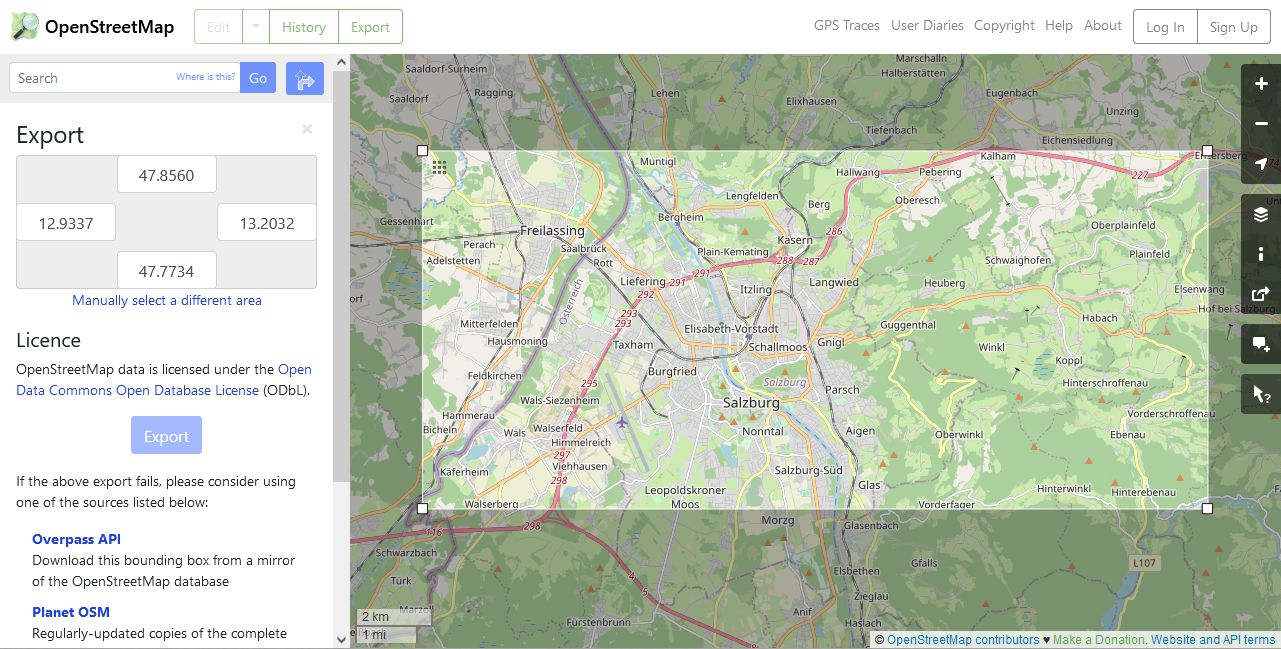
\includegraphics[width=0.9\textwidth]{images/BoundingBoxOSM.png}
 	\caption{
 		Bounding Box for extracted GPS trajectories.
 	}
 	%for reference to this figure
 	\label{figure:BoundingBox}
\end{figure*}

\subsection{Data-set Overview}

Given the bounding box of Salzburg and its surroundings 1.173.334 Data-points were extracted using the OSM Editing API. \footnote{\url{https://wiki.openstreetmap.org/wiki/API_v0.6#GPS_traces}}

The OSM Editing API is a collection of APIs based on RESTful API principles. There are API calls to create, read, update, and delete the three fundamental elements that make up OpenStreetMap's map data. They each return or expect the data for the elements in a XML format.
\autocite[]{wiki:xxx}

The Data-points are returned in a XML format using the GPX standard. \footnote{\url{https://www.topografix.com/GPX/1/1/#type_trksegType}} Important to mention is, that for privacy reasons all waypoints of non-trackable traces are randomized and delivered as one trackSegment. This happens in violation of the GPX standard. 

Get GPS Points: Get /api/0.6/trackpoints?bbox=left,bottom,right,top&page=pageNumber


Use this to retrieve the GPS track points that are inside a given bounding box (formatted in a GPX format).

where:

left, bottom, right, and top are used the same way as they are in the command to retrieve nodes, ways, and relations.

pageNumber specifies which group of 5,000 points, or page, to return. Since the command does not return more than 5,000 points at a time, this parameter must be incremented—and the command sent again (using the same bounding box)—in order to retrieve all of the points for a bounding box that contains more than 5,000 points. When this parameter is 0 (zero), the command returns the first 5,000 points; when it is 1, the command returns points 5,001–10,000, etc.


\subsection{Data Extraction}


\begin{lstlisting}
<?xml version="1.0" encoding="UTF-8"?>
<gpx version="1.0" creator="OpenStreetMap.org" xmlns="http://www.topografix.com/GPX/1/0">
    <trk>
        <name>osmtrack_KUnrl0ZaKm.gpx</name>
        <desc>desc.</desc>
        <url>/user/exbrick/traces/3444105</url>
        <trkseg>
            <trkpt lat="47.8318200" lon="13.0567170">
                <time>2006-08-22T01:37:05Z</time>
            </trkpt>
            <trkpt lat="47.8325810" lon="13.0567800">
                <time>2006-08-22T01:37:20Z</time>
            </trkpt>
            <trkpt lat="47.8331180" lon="13.0569120">
                <time>2006-08-22T01:37:30Z</time>
            </trkpt>
            
\end{lstlisting}




\section{Model & Implementation}
Provide implementation details such as the used software and our software architecture, highlight your own solutions to encountered difficulties. Describe relevant iterations of your implementation.

Providing a route proposal starts further than analyzing geo-located trajectories. Precautious steps were needed in building the architecture to understand the data used for the newly suggested route. 

Therefore a Map Application was created to visualize the extracted and classified data, the routes used for the comparison, and the new suggested routes from the utilized routing engine. Said Map Application is a standalone React App using the Mapbox Plattform for map creation and route visualization. \footnote{\url{https://www.mapbox.com/}} For working with React, Mapbox provides mapbox-gl-js, a javascript library that uses WebGL to render interactive maps from vector tiles and Mapbox styles. \footnote{\url{https://docs.mapbox.com/mapbox-gl-js/guides/}}

For the map and route visualization to interact with the extracted geo trajectory data, a NodeJS backend was developed. The backend interacts with the OSM API and the established Geo-Database, handling the trajectories extraction, classification, and transformation.

With its geospatial data support, MongoDB was selected as the Geo-Database and stores the extracted Data-Set and the further classified data objects. Even though PostGIS \footnote{\url{http://postgis.net/}} is more mature and built on the Open Geospatial Consortium (OGC) standards, the uncertainty of incomplete data sets from the OSM project led to the decision to use the document-based solution.

To work with the OSM project and its map data, the JOSM (Java OpenStreetMap editor) was used to interact with the map layer as the basis for the route proposal. \footnote{\url{https://josm.openstreetmap.de/}}


% https://wiki.openstreetmap.org/wiki/Bounding_Box

Data Extraction

% https://www.topografix.com/GPX/1/1/#type_trksegType

Data Conversion

% https://github.com/mapbox/togeojson

Database

Working with Geodata there is 

MongoDB & Mongoose



Data Prepocessing

TurfJS

Routing Engine

nominatim

osrm

Mapbox API

\section{}

\section{Evaluation}
Describe your methodology. How did you evaluate your work? Why did you choose this methodology? Present results of your evaluation here.

\section{Discussion}
Discuss your results to answer your research question. Does your data support you hypotheses? Put your results into perspective by situating it in the research field/related work.

\section{Conclusion and Future Work}
Summarize your work, outline limitations and future work. 

% \section{Formatierung}
% \label{section:Formatting}

% Text mit beliebigen Sonderzeichen in UTF-8 ohne BOM \ldots
% ,
% \textbf{hervorgehobener Text},
% \texttt{void}\footnote{Fußnote 1},
% mathematische Formel im Text $\sum_{i=0}^n i^2$
% \ldots

% Referenz auf Unterabschnitt \ref{subsection:Coding} der Arbeit, automatisch richtig nummeriert.

% \textcite[]{Mulloni:2010} für einen einen Literaturverweis im laufenden Text.

% Literaturverweise sind essentiell für eine wissenschafliche Arbeit. \autocite[]{McConnell:2004:CCS:1096143}.

% Achtung: nur zitierte Literatur wird im Literaturverzeichnis
% angeführt.\footnote{Fußnote 2}


% Wir verwenden \LaTeX\footnote{ \url{http://en.wikibooks.org/wiki/LaTeX}} -- und das
% ist keine Quelle, sondern blos eine URL.

% \subsection{Figures machen was sie wollen}

% % h = try to place the figure Here
% % t = try to place the figure at the Top of a page
% % p = try to place this figure along with others on a separate Page
% % Note that LaTeX has a sophisticated ranking algorithm to place figures.
% % It is not always easy to accept LaTeX's placing but it is harder doing it
% % manually. Just let it go ;-)
% \begin{figure}[!ht]
% 	\centering
% 	\subfloat[Das Julia Fraktal]{
% 		\includegraphics[width=0.75\linewidth]{images/Julia-Fractal.png}
% 		%for reference of this subfigure only
% 		\label{subfigure:Julia-Fractal}
% 	}
% 	\qquad
% 	\subfloat[Noise für Tinteneffekte]{
% 		\includegraphics[width=0.75\linewidth]{images/Perlin-Coherent.png}
% 		%for reference of this subfigure only
% 		\label{subfigure:Perlin-Coherent}
% 	}
% 	\caption[
% 		Verschiedene Pixelgraphiken\newline
% 		% source url given in the table of figures
% 		\small\texttt{https://mediacube.at/wiki/}
% 	]{
% 		Verschiedene Pixelgraphiken
% 	}
% 	%for reference to all subfigures
% 	\label{figure:PixelImages}
% \end{figure}

% Unterstützte Pixelgraphikformate: PNG, JPEG, PDF.
% Angabe von height oder width meist wichtig.

% Referenz auf Abbildung \ref{figure:PixelImages} mit allen Teilbildern.
% Referenz auf Unterabbildung \ref{subfigure:Julia-Fractal}.

% %figure* stretches figure over both columns
% \begin{figure*}[t]
% 	\centering
% 	\includegraphics[width=0.9\textwidth]{images/KappaGamma.pdf}
% 	\caption{
% 		Vektorgraphik mit \LaTeX\ Beschriftung ($\kappa$, $\gamma$)
% 	}
% 	%for reference to this figure
% 	\label{figure:KappaGammaTau}
% \end{figure*}

% Referenz auf Abbildung \ref{figure:KappaGammaTau}.

% Bei Vektorgraphik mit \LaTeX\ Beschriftung keine Skalierung mit width oder height verwenden.

% Vektorgraphik mit \LaTeX\ Beschriftung kann etwa mit \texttt{ipe} erstellt werden.

% Unterstütztes Vektorgraphikformat: PDF. EPS muss konvertiert werden.


% \subsection{Unterabschnitt 2}
% %for references to this subsection
% \label{subsection:Coding}

% \begin{lstlisting}[
% 	label=listing:Main, %for reference to this listing
% 	float=h,
% 	caption=main.cpp,
% 	firstnumber=10
% ]
% int main(void) {
% 	while (true) {
% 	}
% 	return 0;
% }
% \end{lstlisting}

% Wie man in Listing \ref{listing:Main} in Zeile 10 sieht, kann man die Zeilennummern im Listing absichtlich setzen, hier z.B. auf 10. In Listing \ref{listing:closure} wurde davon nicht Gebrauch gemacht. In diesem Fall beginnt die Nummerierung bei 1.

% \begin{lstlisting}[
%     label=listing:closure,
% 	float=h,
% 	caption=Closure in Javascript,
% 	language=JavaScript
% ]
% function foo(x,y) {
%     let i = x;
%     return function(a) {
%         return i * 2;
%     }
% }
% \end{lstlisting}


% \subsubsection{Unterunterabschnitt i}

% Wörtliches Zitat:
% %select proper language if not in German
% \selectlanguage{english}
% \begin{quote}
% ``Erwin Unruh discovered that templates can be used to compute
% something at compile time. [...] The intriguing part of this exercise, however, was that the production of the prime numbers was performed by the compiler during the compilation process and not at run time.''

% \autocite[305]{Bosch2014}
% \end{quote}
% %select German again or the language that you were using before (note ngerman stands for New German)
% %\selectlanguage{ngerman}
% \selectthesislanguage


% \subsection{Unterabschnitt b}

% \begin{enumerate}
% 	\item Punkt 1
% 	\begin{enumerate}
% 		\item Unterpunkt 1
% 		\item Unterpunkt 2
% 	\end{enumerate}
% 	\item Punkt 2
% \end{enumerate}

% \begin{itemize}
% 	\item Punkt 1
% 	\begin{itemize}
% 		\item Unterpunkt 1
% 		\item Unterpunkt 2
% 	\end{itemize}
% 	\item Punkt 2
% \end{itemize}


% \subsection{Unterabschnitt c}

% \begin{table}[ht]
% 	\centering
% 	\begin{tabular}{r|rrr}
% 		    & $i$ & $j$ & $k$ \\ \hline
% 		$i$ &$-1$ & $k$ &$-j$ \\
% 		$j$ &$-k$ &$-1$ & $i$ \\
% 		$k$ & $j$ &$-i$ &$-1$
% 	\end{tabular}
% 	\caption{
% 		Multiplikationstabelle für Quaternionen
% 	}
% 	\label{table:Quaternions}
% \end{table}

% Referenz auf Tabelle \ref{table:Quaternions}.

% \section{Abschnitt 2}
% \label{section:MathematicalStuff}

% Sei $f(x)$ eine stetige Funktion, so ist die \textbf{Fourier Transformierte}
% $F(\omega)$ wie folgt definiert:
% \begin{equation}
% \label{equation:FourierDefinition}
% 	F(\omega) = \int_{-\infty}^{\infty} f(x) e^{-i\omega t} dt
% \end{equation}

% Referenz auf mathematische Gleichung (\ref{equation:FourierDefinition}).

% Unnummerierte Gleichung:
% \begin{equation*}
% 	e^{i\varphi} = \cos\varphi + i \sin\varphi
% \end{equation*}
% %you may also use \[ \] instead of \begin{equation*} and \end{equation*}

% Gleichungssystem:
% \begin{eqnarray}
% 	g(x) = f(x - x_0) & \Leftrightarrow &
% 		G(\omega) = F(\omega) e^{-i\omega x_0} \\
% 	g(x) = f(x) e^{i\omega_0 x} & \Leftrightarrow &
% 		G(\omega) = F(\omega - \omega_0)
% \end{eqnarray}
